\section{Hello World}

\paragraph{}
   In this part of the document, we're going to be touching on one of the foundational elements in teaching the C programming language: the `Hello World'
   program. Simply put, we are going to write a program that prints the line ``Hello, world!'' into the terminal where we can see it. For the sake of
   simplicity, each figure in this document will be done in Visual Studio Code, but I will, from time to time, include examples from other editors to
   show what may need to be done differently to achieve the same or similar result.

\paragraph{}
   In order to accomplish this, we must first open our text editor and our command line interface (terminal) if they aren't already open. With those
   programs up and running, we must create the file that our code will reside in:

\begin{figure}[h!]
   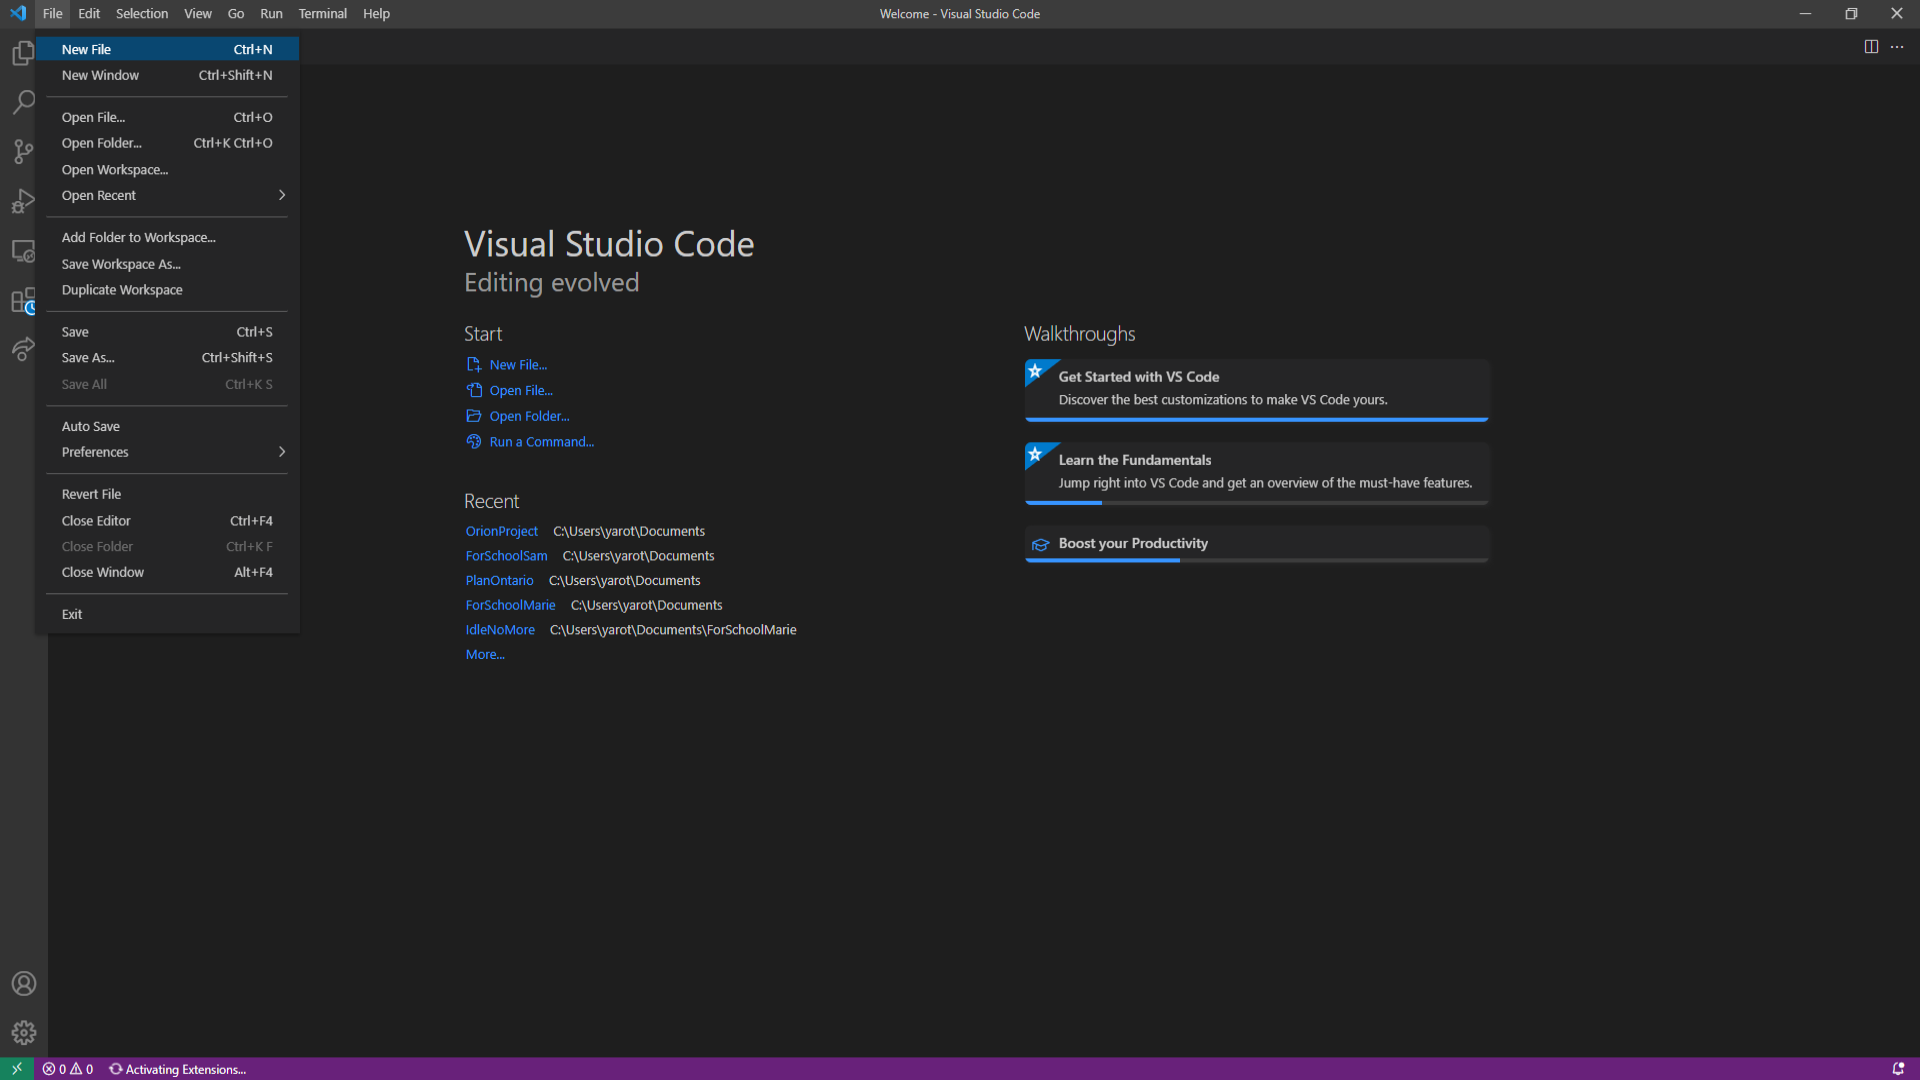
\includegraphics[width=\linewidth]{Figure1_VSCODE.png}
   \caption{Create the file by clicking on the ``New File'' button.}
   \label{fig:vscode_newfile}
\end{figure}

\paragraph{}
   Once the new file is created, we can begin by writing a few lines of code.

\begin{lstlisting}

\end{lstlisting}
